\documentclass[12pt]{../notes}

% Command for Questions
%\question{}

% Command for Notes
% \note{}

% Code to create a minipage where you can type in class notes. 
%%\begin{minipage}[l][2cm][c]{\textwidth}
%\begin{comment}

%\end{comment}
%%\end{minipage}


% Begin Document
%==============================================================================
\begin{document}
% Include the Title of the Handout
\ntitle{6.1: Introduction to Time Series}

\question{Suppose you are trying to predict monthly revenue using historical revenue data. You fit an AR(2) model which you try to use to predict revenue in the same month in the following year. What, if any, issues might you encounter with this prediction?}

\begin{minipage}[l][5cm][c]{\textwidth}
%\begin{comment}
\note{
\begin{itemize}
\item \textbf{Autocorrelation does not aid prediction.} Our model assumes that only the previous two lags are useful in the next prediction. Given that we are trying to predict 12 lags into the future, we simply don't have any observations to inform our time series so we will simply predict the average trend or difference. 
\item \textbf{Even trend prediction will not be reliable:} The prediction is far enough into the future to cast doubt on whether historical trends will continue. The estimated value is likely unreliable. 
\end{itemize}
}
%\end{comment}
\end{minipage}

\nspace

\question{Describe, in your own words, the difference between a time dependent \textit{trend} and time-dependent \textit{autocorrelation.} Can you have both at the same time?}

\begin{minipage}[l][5cm][c]{\textwidth}
%\begin{comment}
\note{A time dependent trend means that the \textit{average} value of Y is associated with time. A time dependent autocorrelation means that individual values of Y taken closely in time tend to vary together above or below the average. You can certainly have a time dependent trend and autocorrelation at the same time. For example, house prices in Utah tend to generally rise over time (time dependent trend). However, after accounting for the general rise in prices, home price increases tend to come in waves based on the current economic conditions. Those waves could reveal some time dependent autocorrelations.} 
%\end{comment}
\end{minipage}

\nspace

\question{Using the table on page 5 of the 6.1 notes, which model type would you recommend based on the output provided in Figure \ref{ar_example1}?}

\begin{minipage}[l][3cm][c]{\textwidth}
%\begin{comment}
\note{AR(2) (though the PACF cuts off at lag 3, perhaps suggesting an AR(3) model which is not discussed in the table). }
%\end{comment}
\end{minipage}

\nspace
\question{Using the table on page 5 of the 6.1 notes, which model type would you recommend based on the output provided in Figure \ref{ar_example2}?}

\begin{minipage}[l][3cm][c]{\textwidth}
%\begin{comment}
\note{NO MODEL: The ACF plot suggests the time series is not stationary. }
%\end{comment}
\end{minipage}

\begin{figure}
\centering
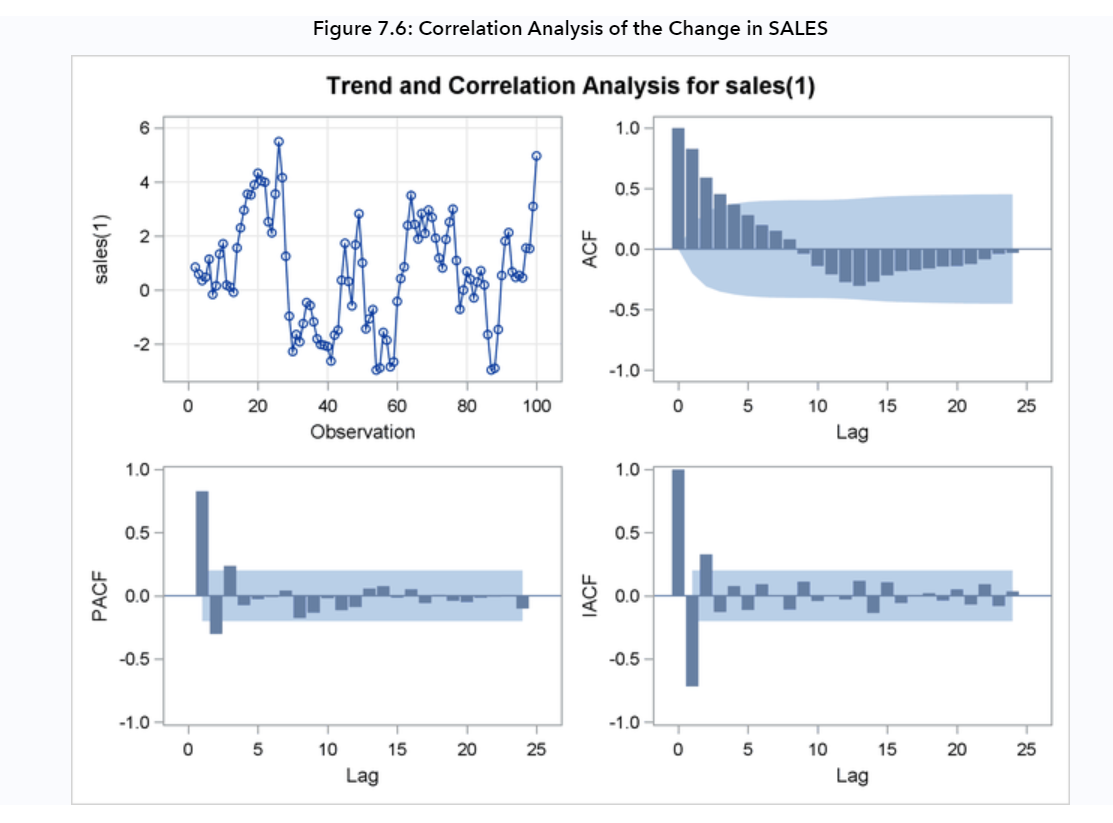
\includegraphics[width=\textwidth]{../figures/module6/acf_example1.png}
\caption{Sample ARMA model output.}
\label{ar_example1}
\end{figure}

\begin{figure}
\centering
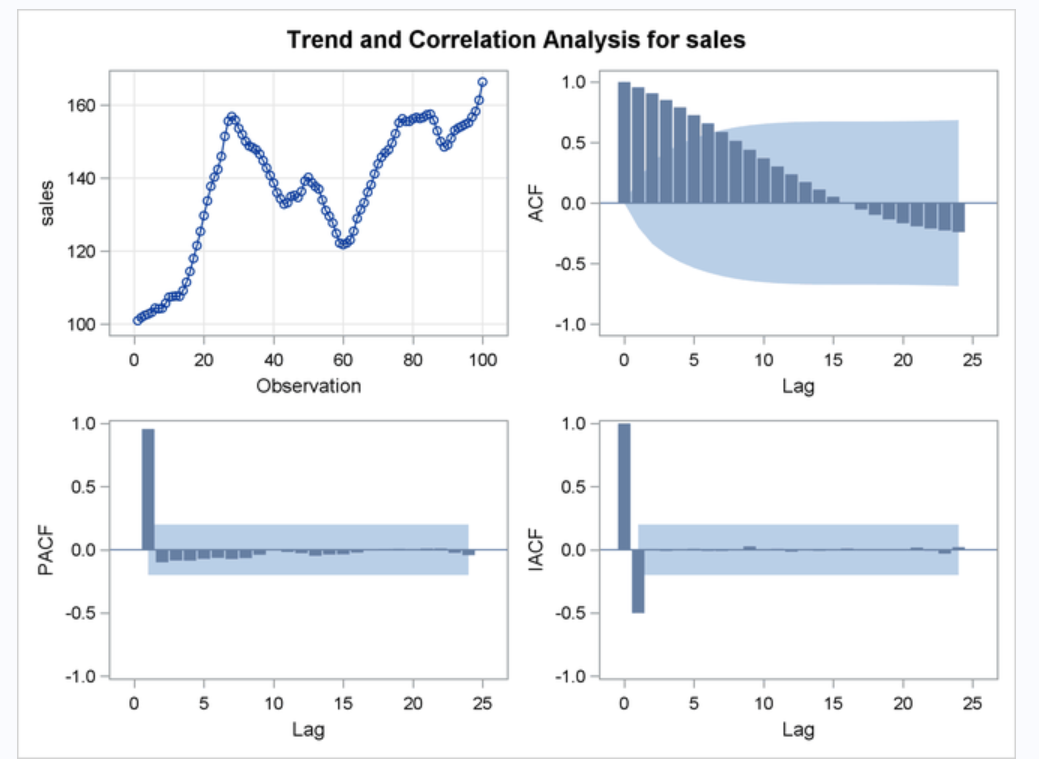
\includegraphics[width=\textwidth]{../figures/module6/acf_example2.png}
\caption{Sample ARMA model output.}
\label{ar_example2}
\end{figure}




\end{document}